\chapter{Implementación} \label{chap:implementacion}
\begin{tcolorbox}[colback=red!5!white,colframe=red!75!black]
AQUÍ HABLAR DE CONCEPTOS RELACIONADOS CON LA CARRERA: DISEÑO JERÁRQUICO, =! CAPAS, LISTAS DE ACCESO..
\end{tcolorbox}

Nos basaremos en la versión\textit{ Queens }de OpenStack que es la versión estable más actualizada hasta la fecha \cite{noauthor_releases:_nodate}.

\section{Desplegando OpenStack}
En este punto vamos a ver las opciones que tenemos para implementar nuestra nube IaaS con OpenStack y como lo haremos finalmente con el uso de una todo en uno (\textit{all-in-one}). Eso significa que  los diferentes servicios de OpenStack se ejecutarán en la misma máquina, que puede ser una máquina física o una máquina virtual y servirá de guía para implementar OpenStack en Ubuntu.

\subsection{Métodos de despliegue}\label{subsesc:metodosdespliegue}
OpenStack se puede implementar de varias maneras:

\begin{itemize}
\item Manualmente. OpenStack se puede implementar manualmente mediante la aplicación de los pasos descritos en la documentación pertinente \cite{noauthor_install_nodate}.
\item Scripted. También se puede implementar de forma guiada mediante el uso de una solución como Packstack o DevStack, que será la que nosotros usemos.
\item Despliegue a gran escala. Otra opción es el despliegue de OpenStack a gran escala, utilizando soluciones de implementación más avanzadas, como Triple O, Director \cite{noauthor_tripleo_nodate}\cite{noauthor_director_nodate}.
\end{itemize}

\subsection{El rol de los tipos de nodo}\label{subchap:rol-nodos}
Normalmente, existen diferentes roles según el tipo de nodo en una nube de OpenStack como vemos en la Fig.\ref{nodos} Los roles que se utilizan dependen de la configuración existente:

\begin{figure}
    \centering
    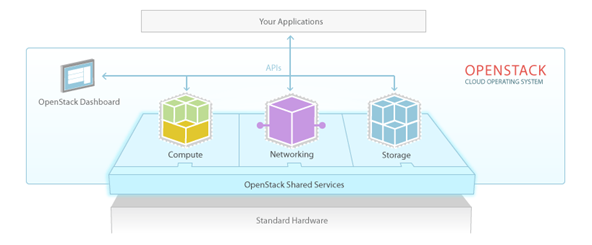
\includegraphics[width=0.7\textwidth]{imagenes/capitulo6/nodos.png}
    \caption{Tipos de nodos en OpenStack.}
	\vspace{0.3cm}
    \footnotesize{Fuente: OpenStack wiki}
    \label{nodos}
\end{figure}

\begin{itemize}
\item Nodo controlador (\textit{Controller node}). Ejecuta los servicios de control. En este nodo encontraremos servicios como Keystone , la cola de mensajes, la base de datos MariaDB y todo lo esencial para controlar la nube.
\end{itemize}

\begin{itemize}
\item Nodo controlador de red (\textit{Network controller node}).  Proporciona servicios de red a la nube. Es el tipo de no que proporciona SDN y está conectado a redes internas y externas.
\end{itemize}

\begin{itemize}
\item Nodo de cómputo (\textit{Compute nodes}). Son los nodos que realmente van a ejecutar las instancias en OpenStack. Básicamente, los compute nodes son los hipervisores y en ellos algunas partes de Nova se están ejecutando para interactuar con el hipervisor, lo que permite a OpenStack programar el funcionamiento de máquinas virtuales en un nodo de cómputo específico.
\end{itemize}

\begin{itemize}
\item Nodos de almacenamiento (\textit{Storage nodes}). Los nodos de almacenamiento son todo lo que involucra  el almacenamiento de objetos (servicios como Swift o Ceph) y en un clúster de almacenamiento avanzado, estamos hablando fácilmente de docenas de storage nodes para garantizar la disponibilidad del mismo.
\end{itemize}

Aunque hagamos referencia a un nodo, en un entorno en producción redundante podrá haber tantos como sean necesarios de cada tipo para asegurar alta disponibilidad. 

\subsection{Despliegues con Devstack}
\textit{DevStack} es la solución estándar para la creación de un entorno de pruebas con OpenStack y se ejecuta en múltiples distribuciones de Linux incluyendo Ubuntu, Fedora, OpenSUSE, Debian, CentOS o RedHat entre otras. DevStack proporciona una serie de scripts para montar un entorno OpenStack completo basado en la configuración que especificaremos en un archivo destinado a ese fin. 

DevStack es muy popular entre los desarrolladores, ya que se usa para pruebas de desarrollo y operativas. Es importante señalar que DevStack no se creó para su uso en producción.

Se pueden usar diferentes escenarios al configurar un entorno de laboratorio basado en Ubuntu con DevStack:

\begin{itemize}
\item All-in-one Single VM.
\end{itemize}

\begin{itemize}
\item All-in-one Single Machine.
\end{itemize}

\begin{itemize}
\item Multi-node Lab.
\end{itemize}

La dos primeras son la instalación todo en uno con la salvedad de realizarla en un máquina virtual o una máquina física. La última, puede usar varias VMs o máquinas físicas. 

Optaremos por la segunda opción para realizar la implementación de este proyecto por motivos obvios de disponibilidad de equipos y presupuesto, es decir, una configuración all-in-one en una máquina física, lo cual significa que no haremos una distinción estricta entre los tipos de nodos vistos sino que tendremos una máquina en el entorno creado que proporcione las funciones de todos estos nodos.

\section{Proceso de instalación}
Usaremos Ubuntu Server 16.04.3 LTS como sistema operativo. Para ello, el departamento de Telemática cedió dos servidores dedicados ya que en el proceso de instalación se hacen cambios sustanciales en la configuración del equipo y además se requiere de altos requisitos hardware para que el funcionamiento del despliegue sea óptimo.

Vamos a comenzar con la implementación de OpenStack mediante Devstack . El proceso de instalación será similar en ambos servidores con algunas salvedades.

\subsection{Puesta a punto de los servidores}
En primer lugar, una vez instalado en ambos servidores el sistema operativo, haremos una serie de verificaciones. 

Para empezar, necesitamos verificar la memoria RAM disponible, ya que si no tenemos 8 GB como mínimo, la instalación fallará. Inicialmente teníamos 16 GB en el primer servidor y tras la instalación:

\begin{lstlisting}[style=Consola]
jorge@wimunet4::~$ free
         total     used     free   shared  buff/cache  available
Mem:  16298968   5222208  8664664    9464     2412096   10721112
Swap:  2097148        0  2097148
\end{lstlisting}

Y 32 GB en el segundo servidor por lo que esta parte queda cubierta:

\begin{lstlisting}[style=Consola]
jorge@wimunet5:~$ free
         total     used      free   shared  buff/cache  available
Mem:  32610848  1025700  26423112   361292     5162036   30669864
Swap: 33221628        0  33221628
\end{lstlisting}

Puesto que los servidores están dentro de la ETSIIT, tras solicitar una IP pública se nos asignó la 150.214.190.177. Una vez obtenida configuramos el Servidor 1 modificando el archivo /etc/network/interfaces de nuestra máquina como sigue:

\begin{lstlisting}[style=Consola]
jorge@wimunet4::~$ cat /etc/network/interfaces
# interfaces(5) file used by ifup(8) and ifdown(8)
auto lo
iface lo inet loopback
	
auto enp3s0
iface enp3s0 inet static
	address 150.214.190.177
	netmask 255.255.254.0
	gateway 150.214.190.222
	dns-nameservers 150.214.204.10

auto enp3s0:1
iface enp3s0:1 inet static
	address 10.5.1.201
	netmask 255.255.255.0
\end{lstlisting}

De este modo conseguimos:
\begin{itemize}
\item Acceso a Internet con la IP pública 150.214.190.177.
\item Creación de la interfaz virtual \textit{enp3s0:1} que nos permitirá asignar a las instancias que creemos IPs flotantes (ver sección \ref{subsec:IP-flotante}) dentro de la red 10.5.1.201/24 para su acceso desde el exterior resolviendo así la problemática de tener una única IP pública.
\end{itemize}

De forma análoga modificamos las interfaces del Servidor 2 para acceder al exterior a través del Servidor 1 y tener también la posibilidad de asignar IPs flotantes en la red 10.5.3.201/24 creando la interfaz \textit{enp0s31f6:2}:

\begin{lstlisting}[style=Consola]
iface enp0s31f6 inet static
        address 10.5.2.2
        netmask 255.255.255.0
        gateway 10.5.2.1
        dns-nameservers 150.214.204.10
        dns-search ugr.es

auto enp0s31f6:2
iface enp0s31f6:2 inet static
        address 10.5.3.201
        netmask 255.255.255.0
\end{lstlisting}

Como comentamos en el capítulo anterior, para conectar ambos servidores se instaló una tarjeta de red en el Servidor 1 para comunicar ambos servidores a través de la red 10.5.2.0/24. 

Así en el Servidor 1 disponemos de una interfaz nueva con la IP 10.5.2.1:

\begin{lstlisting}[style=Consola]
jorge@wimunet4:~$ ifconfig enx6038e0e3083f
enx6038e0e3083f Link encap:Ethernet  HWaddr 60:38:e0:e3:08:3f
          inet addr:10.5.2.1  Bcast:10.5.2.255  Mask:255.255.255.0
          inet6 addr: fe80::6238:e0ff:fee3:83f/64 Scope:Link
          UP BROADCAST RUNNING MULTICAST  MTU:1500  Metric:1
          RX packets:1134037 errors:0 dropped:0 overruns:0 frame:0
          TX packets:1747042 errors:0 dropped:0 overruns:0 carrier:0
          collisions:0 txqueuelen:1000
          RX bytes:89409470 (89.4 MB)  TX bytes:2337586769 (2.3 GB)
\end{lstlisting}

Y en el Servidor 2, asignamos a la tarjeta de red la IP 10.5.2.2:

\begin{lstlisting}[style=Consola]
jorge@wimunet5:~$ ifconfig enp0s31f6
enp0s31f6 Link encap:Ethernet  HWaddr 2c:fd:a1:6e:c3:cf
          inet addr:10.5.2.2  Bcast:10.5.2.255  Mask:255.255.255.0
          inet6 addr: fe80::2efd:a1ff:fe6e:c3cf/64 Scope:Link
          UP BROADCAST RUNNING MULTICAST  MTU:1500  Metric:1
          RX packets:721537 errors:0 dropped:0 overruns:0 frame:0
          TX packets:490297 errors:0 dropped:0 overruns:0 carrier:0
          collisions:0 txqueuelen:1000
          RX bytes:929277285 (929.2 MB)  TX bytes:51982744 (51.9 MB)
          Interrupt:20 Memory:92f00000-92f20000
\end{lstlisting}

\subsection{Verificaciones sobre la configuración de los servidores}
Una vez preparados ambos servidores queda realizar algunas pruebas de conexión:

\begin{itemize}
\item Conectividad entre ambos servidores:
\end{itemize}
\begin{lstlisting}[style=Consola]
jorge@wimunet4:~$ ping 10.5.2.2
PING 10.5.2.2 (10.5.2.2) 56(84) bytes of data.
64 bytes from 10.5.2.2: icmp_seq=1 ttl=64 time=0.250 ms
64 bytes from 10.5.2.2: icmp_seq=2 ttl=64 time=0.201 ms
^C
--- 10.5.2.2 ping statistics ---
2 packets transmitted, 2 received, 0% packet loss, time 999ms
rtt min/avg/max/mdev = 0.201/0.225/0.250/0.028 ms

\end{lstlisting}

\begin{itemize}
\item Conexión del Servidor 1 a la red pública:
\end{itemize}
\begin{lstlisting}[style=Consola]
jorge@wimunet4:~$ ping www.google.es
PING www.google.es (216.58.201.163) 56(84) bytes of data.
64 bytes from mad08s06-in-f3.1e100.net (216.58.201.163): icmp_seq=1 ttl=54 time=12.2 ms
64 bytes from mad08s06-in-f3.1e100.net (216.58.201.163): icmp_seq=2 ttl=54 time=12.2 ms
^C
--- www.google.es ping statistics ---
2 packets transmitted, 2 received, 0% packet loss, time 1001ms
rtt min/avg/max/mdev = 12.239/12.251/12.264/0.111 ms

\end{lstlisting}

\begin{itemize}
\item Conexión del Servidor 2 a la red pública:
\end{itemize}
\begin{lstlisting}[style=Consola]
jorge@wimunet5:~$ ping www.google.es
PING www.google.es (172.217.16.227) 56(84) bytes of data.
64 bytes from mad08s04-in-f3.1e100.net (172.217.16.227): icmp_seq=1 ttl=53 time=13.1 ms
64 bytes from mad08s04-in-f3.1e100.net (172.217.16.227): icmp_seq=2 ttl=53 time=13.0 ms
^C
--- www.google.es ping statistics ---
2 packets transmitted, 2 received, 0% packet loss, time 1001ms
rtt min/avg/max/mdev = 13.052/13.096/13.141/0.122 ms
jorge@wimunet5:~$
\end{lstlisting}

Para que esta última conexión sea posible, en el Servidor 1 creamos un script en bash llamado \textit{network\_to\_second\_pc.sh} para permitir la conexión del Servidor 2 hacia Internet a través del Servidor 1 que es el que está conectado a la toma de la red externa.

\begin{lstlisting}[style=Consola]
jorge@wimunet4:~$ cat network_to_second_pc.sh
ifconfig enx6038e0e3083f 10.5.2.1/24
iptables -t nat -A POSTROUTING -o br-ex -j MASQUERADE
\end{lstlisting}

Como vemos, en él estamos creando una regla con el firewall \textit{iptables} para hacer \textit{postrouting} mediante NAT (\textit{Network Address Translation}) a través de la interfaz \textit{br-ex} que es la que nos da acceso en el Servidor 1 a la red pública.

\subsection{Instalando OpenStack}\label{sec:instalacion}
En este punto nos encontramos ya en disposición de instalar OpenStack. 

En primer lugar vamos a ver la parte que es idéntica para ambos servidores comenzando por la creación de un usuario con el nombre \textit{stack} y permisos de administrador:

\begin{lstlisting}[style=Consola]
jorge@wimunet4:~$  sudo useradd -s /bin/bash -d /opt/stack -m stack; echo "stack ALL=(ALL) NOPASSWD: ALL"| sudo tee /etc/sudoers.d/stack; sudo su - stack
\end{lstlisting}

A continuación, instalamos los paquetes \textit{cloud-init} que contienen un  conjunto de paquetes que son útiles cuando se trabaja con DevStack en una máquina Ubuntu. Básicamente son scripts de Python, Git y algunos más.

\begin{lstlisting}[style=Consola]
stack@wimunet4:~$ sudo apt-get install cloud-init
\end{lstlisting}

En esta parte de la configuración, pasamos a clonar todos los paquetes actuales de OpenStack  que están disponibles en Git \cite{noauthor_devstack:_2018} a la máquina local, con lo que conseguiremos poder comenzar con la instalación en la misma. Además indicamos que la versión que queremos instalar sea Queens.

\begin{lstlisting}[style=Consola]
stack@wimunet4:~$ git clone https://git.openstack.org/openstack-dev/devstack -b stable/queens
\end{lstlisting}

Tras esto, se habrá creado un directorio llamado \textit{devstack}:

\begin{lstlisting}[style=Consola]
stack@wimunet4:~$ cd devstack
\end{lstlisting}

Dentro de él existen distintos archivos, los que más nos interesarán son \textit{stack.sh, unstack.sh y clean.sh}, que se utilizan para instalar, desinstalar, y limpiar la configuración existente respectivamente. Necesitamos crear un archivo \textit{ local.conf}, al que antes hacíamos referencia y  que contendrá la configuración necesaria para que la instalación se realice acorde a nuestra necesidades. 

Este archivo será distinto para cada servidor. El archivo de configuración del Servidor 1 lo podemos ver en el apéndice \ref{sec:ConfServer1} y para el Servidor 2 en el \ref{sec:ConfServer2}.

Una vez creados ambos archivos podemos ya ejecutar el script \textit{stack.sh}, que leerá los parámetros de configuración de \textit{local.conf} y construirá nuestra IaaS multi-región con DevStack OpenStack basándose en estos parámetros.

\begin{lstlisting}
stack@wimunet4:~/devstack$ ./stack.sh
\end{lstlisting}

\begin{figure}
    \centering
    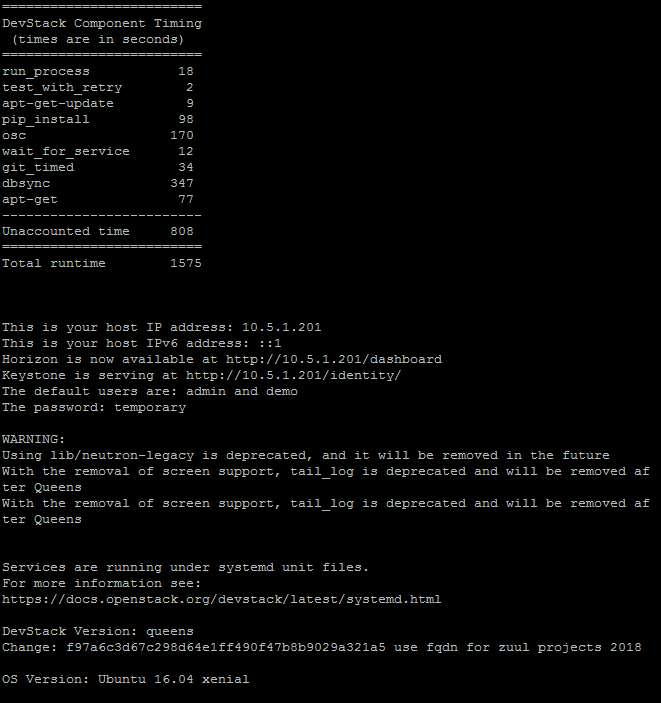
\includegraphics[width=1\textwidth]{imagenes/capitulo6/finInstalacionServer1.png}
    \caption{Reporte de la instalación.}
	\vspace{0.3cm}
    \label{fininstallserver1}
\end{figure}

El tiempo promedio de ejecución del script es largo y dependerá de la capacidad  del hardware de nuestro servidor. Cuando finaliza la instalación de manera correcta, nos mostrará un reporte de la misma, Fig.\ref{fininstallserver1}.
En el podemos ver el tiempo que ha demorado cada componente, nuestra dirección IPv4 e IPv6 y como se ha creado un usuario \textit{demo} que será un tenant además del usuario administrador, \textit{admin}. Por último, podemos ver que la versión instalada es \textit{Queens}, como ya hemos comentado, la versión estable más reciente que incorpora versiones actualizadas de los proyectos de OpenStack.\cite{noauthor_queens_nodate}

Después de implementar OpenStack en Ubuntu, abrimos un navegador en la dirección IP de la máquina donde  acabamos de alojar OpenStack, cuya IP pública es 150.214.190.177, en caso de que estemos accediendo a Horizon desde una red externa, mientras que desde el servidor podremos acceder directamente a la IP privada, 10.5.1.201 y conectarnos. Se mostrará entonces la página de la Fig.\ref{login} donde podremos iniciar sesión como admin utilizando la contraseña establecida. 

\begin{figure}
    \centering
    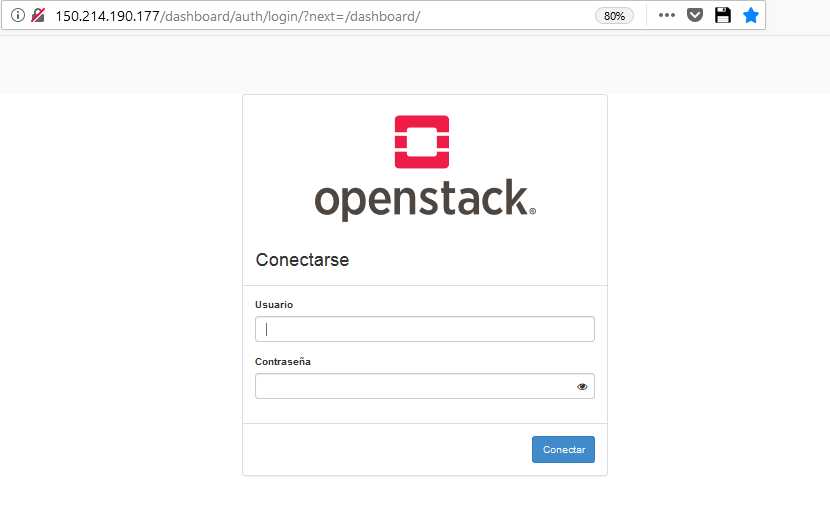
\includegraphics[width=1\textwidth]{imagenes/capitulo6/login.PNG}
    \caption{Página de acceso al dashboard de Horizon.}
	\vspace{0.3cm}
    \label{login}
\end{figure}

\section{Configuración de un escenario mediante Horizon}
Horizon es la herramienta más importante para los administradores que se están iniciando en OpenStack pues proporciona una interfaz web que facilita el trabajo como administrador de OpenStack.

\jorge{La figura 7.4 se ve muy poco, piensa si podrías ponerla en apaisado.}

\begin{figure}
    \centering
    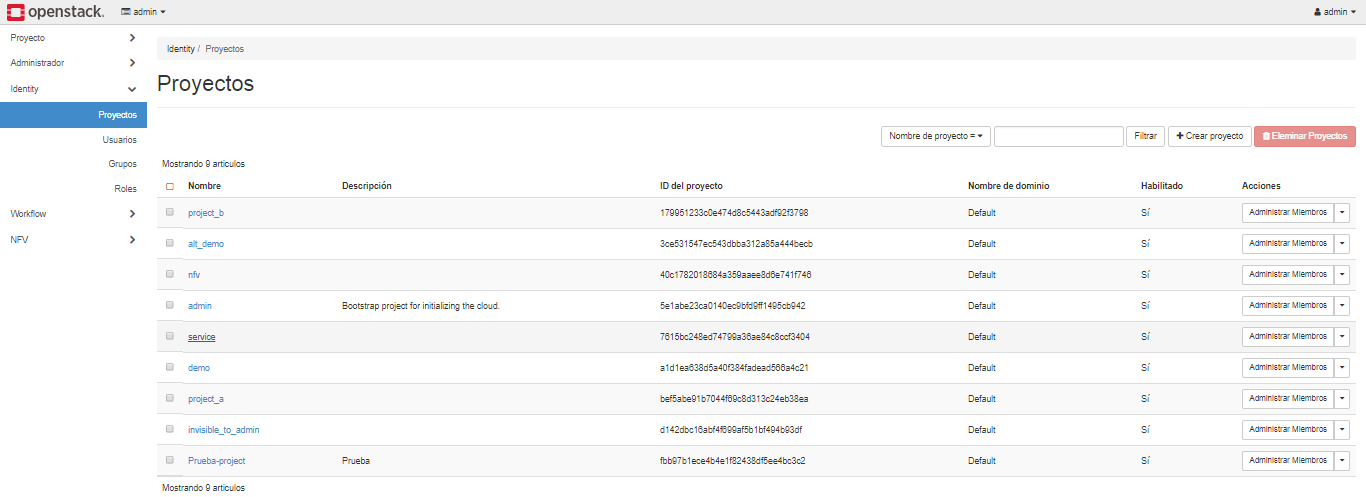
\includegraphics[width=1\textwidth]{imagenes/capitulo6/primeracceso.png}
    \caption{Panel inicial de Proyectos tras acceder a Horizon.}
	\vspace{0.3cm}
    \label{primeracceso}
\end{figure}

En este apartado procederemos con la implementación de instancias desde la interfaz web de Horizon. Trataremos el propósito y uso de tenants, usuarios y roles, diferenciaremos entre ámbitos administrativos en Horizon y discutiremos los componentes necesarios para implementar instancias. Veremos lo fácil que resulta desplegar instancias y también sus implicaciones, comenzando con la creación de un proyecto o tenant y acabando con una cloud operativa.

Antes de acceder a la interfaz web, vamos a ver el estado del servidor web Apache. Los repositorios de Ubuntu, incluyen el servidor de código abierto Apache, el más utilizado en sistemas operativos Linux. Apache sirve las páginas web a los navegadores de los usuarios al acceder a la dirección IP o al nombre de dominio asociado a nuestro sistema Ubuntu. Además Apache se ejecuta en segundo plano como un servicio del sistema, lo que significa que podemos iniciarlo, detenerlo y reiniciarlo usando el servicio nativo de comandos en Ubuntu. Para iniciar y comprobar su estado podemos escribir en un terminal:

\begin{lstlisting}
stack@wimunet4:~/devstack$ sudo service apache2 start
stack@wimunet4:~/devstack$ sudo service apache2 status
\end{lstlisting}

Nuestro servidor web Apache aloja Horizon, es decir, los procesos del Dashboard. El servidor web está activo y ejecutándose, lo que significa que podemos ir a la interfaz web y ver qué aspecto tiene Horizon.

Abriendo un navegador web, Firefox en mi caso, podremos conectarnos a la dirección IP del servidor web Horizon usando la IP pública 150.214.190.177, como ya vimos en la última parte del apartado anterior. 

Firefox resuelve automáticamente el nombre DNS de Horizon. En el prompt de inicio de sesión, podemos iniciar sesión como usuario administrador. Como todavía no hemos creado nada, solo hay un usuario disponible, el usuario administrador con las contraseñas que proporcionamos. En realidad también hay instalado un cliente de demostración, demo, con el que podremos iniciar igualmente sesión como un usuario cliente pero que no usaremos. 

Tras introducir las credenciales para el usuario \textit{admin} accederemos al escritorio donde se nos mostrará el panel de la Fig.\ref{primeracceso} en el que podemos ver un listado de los proyectos que existen en nuestro entorno.

De modo que en Horizon existen diferentes puntos de vista. Si somos administradores de OpenStack, veremos diferentes elementos que si nos autenticamos como un usuario tenant. El usuario tenant solo ve el entorno para ese tenant específico, mientras que el usuario administrador, puede ver todos los entornos.

Una de las partes más importante para el usuario administrador es la pestaña de identidad, “Identity”. Una de las primeras cosas que haremos como administrador será crear un entorno donde los tenants puedan iniciar sesión, como veremos después.

Además, está la pestaña de administración “Administrador”, en la que el administrador puede gestionar la infraestructura de la nube, infraestructura en la que están disponibles los hipervisores o \textit{Host Agrgregates}, que es un grupo de hipervisores, las imágenes de Glance para arrancar instancias, o bien gestionar las redes públicas. Estas son típicamente las tareas administrativas.  
También tenemos una pestaña de proyectos, “Proyecto”, que no es algo en lo que se trabajará como administrador, porque normalmente se separará entre el entorno del tenant, que contiene el entorno en el que van a derivar las máquinas virtuales y el entorno de administración, que realmente está destinado a proporcionar infraestructura.

Antes de comenzar a trabajar en Horizon, vamos a familiarizarnos con algunos conceptos esenciales de OpenStack:

\begin{itemize}
\item \textbf{Service}. Un servicio es un proyecto. Es un componente esencial de OpenStack, tal como lo define OpenStack Foundation.
\end{itemize}


\begin{itemize}
\item \textbf{Tenant}. Un tenant es un cliente. Si OpenStack se usa como una nube pública, se pueden crear varios tenants. También se conoce como proyecto.
\end{itemize}


\begin{itemize}
\item \textbf{Role}. Con un rol, nos referimos a un conjunto de permisos que se usan para permitir a los usuarios hacer lo que necesiten.
\end{itemize}


\begin{itemize}
\item \textbf{User}. Un usuario es una entidad administrativa que ha sido asignada a un rol específico en OpenStack.
\end{itemize}

\subsection{Creación de proyectos o tenants}
A continuación vamos a ver cómo crear un tenant desde  Horizon. Normalmente, la primera tarea para el administrador de OpenStack es crear los entornos de tenants, también conocidos como  proyectos, lo cual haremos desde la pestaña “Identity”.

Haciendo clic en la pestaña “Identity” podemos ver que hay cuatro elementos diferentes: los proyectos, los usuarios, los grupos y los roles, como se aprecia en la Fig.\ref{primeracceso}.

Podemos ver que los proyectos activos entre los más relevantes se encuentra el proyecto de administración, “admin”, el proyecto de servicios, “service” y el proyecto para la gestión de NFVs, “nfv”.

Los proyectos que no se vayan a usar como puede ser el caso de “demo” podemos eliminarlos marcando el proyecto y clicando en el botón rojo situado en la parte superior derecha “Eliminar Proyectos”.

El proyecto de administración es donde se encuentra el administrador y el proyecto de servicios es un tenant de los servicios de OpenStack. Esto quiere decir que todos los servicios están creados en un proyecto también, lo cual está relacionado con los permisos, al ponerlos todos en un proyecto específico, es fácil darles acceso a estos servicios a los distintos tenants.

Vamos a crear ahora nuestro propio proyecto haciendo clic sobre icono “Crear Proyecto”. De este modo crearemos el entorno donde los usuarios que especifiquemos de la nube puedan crear sus instancias o los recursos que necesiten.

\begin{tcolorbox}[colback=red!5!red,colframe=red!75!black]
QUIZÁS SEA NECESARIO AÑADIR LA MAYORIA DE USUARIOS QUE APARECEN PARA QUE FUNCIONE COMO DEBE, COMPROBAR ESTO.
\end{tcolorbox}

\begin{figure}
    \centering
    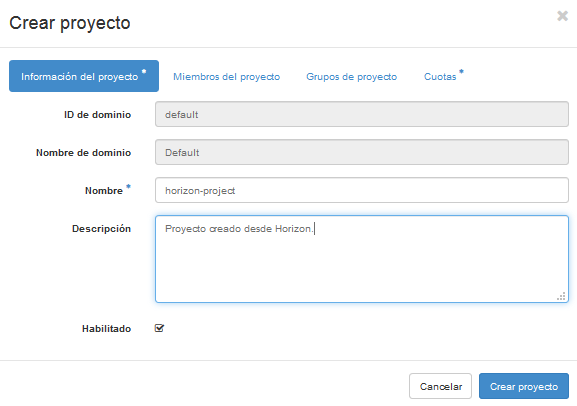
\includegraphics[width=1\textwidth]{imagenes/capitulo6/crear-proyecto-1.PNG}
    \caption{Creación de un proyecto en Horizon.}
	\vspace{0.3cm}
    \label{crear-proyecto-1}
\end{figure}

Vamos a llamarlo “horizon-project”, Fig.\ref{crear-proyecto-1}. La descripción no es necesaria. En las pestañas “Miembros del proyecto” y “Grupos del proyecto” podemos especificar los miembros y grupos del proyecto que deseemos. En este caso dejaremos los que vienen por defecto para después ver como se añaden los que creemos nosotros y no los que se instalaron como demo. Podemos pasar directamente al apartado de “Cuotas”.

La cuota del proyecto es importante ya que se utiliza para determinar que los usuarios de su proyecto no pueden obtener acceso ilimitado a los recursos en la nube. Por lo tanto, podemos limitar la cantidad de instancias, la cantidad de RAM que se puede usar, estableciéndola en 4096 MB por ejemplo, porque tenemos alrededor de 9 GB de RAM solamente tras la instalación de DevStack, la cantidad de direcciones IP flotantes, la cantidad de redes, etc.

Después de imponer las limitaciones que vemos  en la Fig.\ref{crear-proyecto-2}, habremos especificado  las propiedades de cuota del proyecto. Haciendo  clic en “Crear proyecto” crearemos el tenant que se agregará a los que ya existían.

\begin{figure}
    \centering
    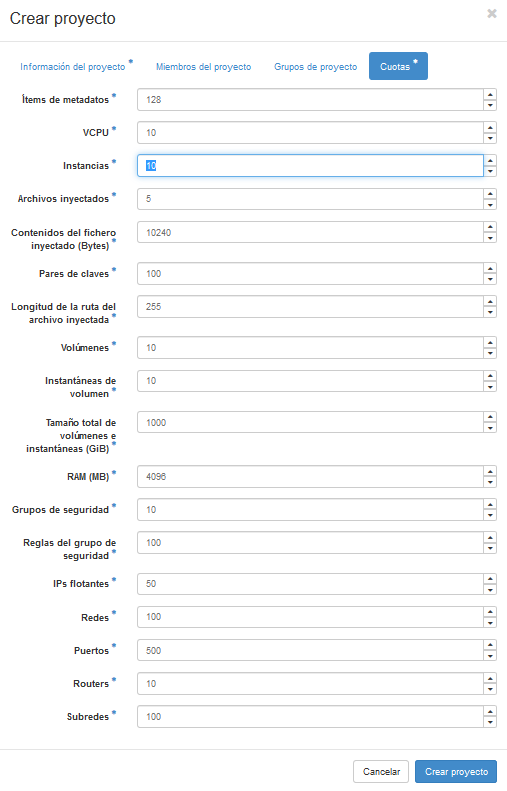
\includegraphics[width=1\textwidth]{imagenes/capitulo6/crear-proyecto-2.PNG}
    \caption{Cuota del proyecto.}
	\vspace{0.3cm}
    \label{crear-proyecto-2}
\end{figure}

\subsection{Creación de usuarios}
El siguiente paso será crear un usuario. Dentro de “Identity” clicamos en “Usuarios” y “Crear usuario”, Fig.\ref{crear-usuario}.

Vamos a darle un nombre, “horizon-user”. No necesitamos una descripción ni un correo electrónico pero sí una contraseña. Los usuarios también deben asignarse a un proyecto, de modo que en la lista “Proyecto principal”, podemos seleccionar el proyecto que acabamos de crear. También podemos definir en el desplegable “Rol”, el tipo de usuario o rol que tendrá. Especificamos que sea \textit{Member}. Un usuario Member puede crear todo lo necesario en el entorno de la nube. Después de especificar las propiedades del usuario, podemos hacer clic en “Crear usuario” y con esto, dicho usuario podrá ya iniciar sesión.

\begin{figure}
    \centering
    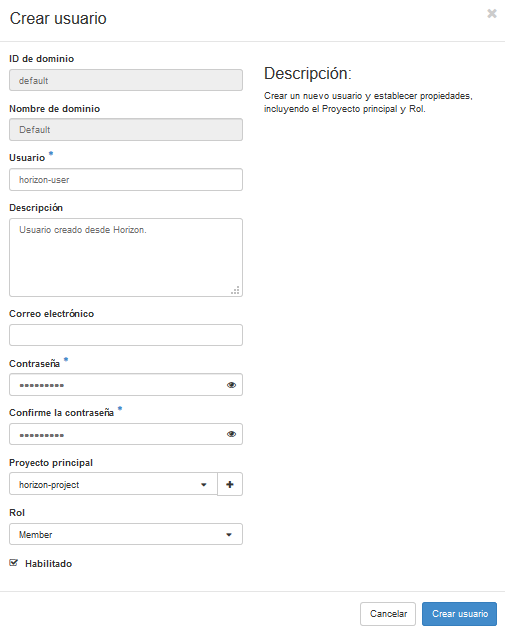
\includegraphics[width=1\textwidth]{imagenes/capitulo6/crear-usuario.PNG}
    \caption{Creación de un usuario.}
	\vspace{0.3cm}
    \label{crear-usuario}
\end{figure}

Las pestañas “Grupos” y “Roles” de “Identity” se usan con menor frecuencia. Sus funciones son las de  agrupar diferentes usuarios y definir nuevos roles respectivamente, pero normalmente para la mayoría de los entornos en la nube, basta con los roles de miembro y administrador.

\jorge{La figura 7.8 se ve muy poco, ponla en apaisado.}

Si cerramos sesión e iniciamos de nuevo pero esta vez con el usuario “horizon-user” creado, entraremos directamente a la vista general del usuario que vemos en la Fig.\ref{acceso-horizon-user}, donde el proyecto se abre de manera predeterminada y en el que podremos ver un reporte del uso y las capacidades de nuestro entorno cloud en cuanto a instancias, RAM y el resto de recursos principales.

\begin{tcolorbox}[colback=red!5!red,colframe=red!75!black]
ESTAS IMÁGENES QUE HAY QUE METER TAN LARGAS, COMO LA DE LOS ENDPOINTS, PROBAR A HACER LA VENTA MAS PEQUEÑA A VER SI ASÍ SALE MEJOR.
\end{tcolorbox}

\begin{figure}
    \centering
    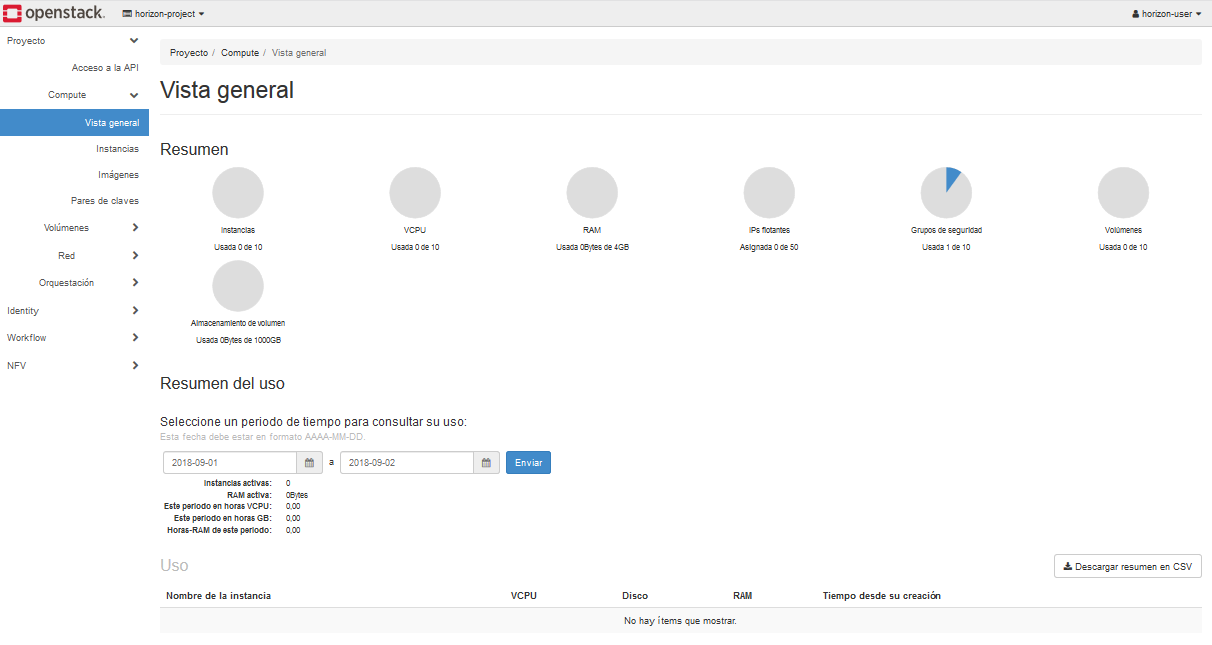
\includegraphics[width=1\textwidth]{imagenes/capitulo6/acceso-horizon-user.PNG}
    \caption{Vista general del proyecto horizon-project.}
	\vspace{0.3cm}
    \label{acceso-horizon-user}
\end{figure}

\subsection{Recursos necesarios para crear una instancia}
En este apartado, vamos a explicar qué se necesita para implementar una instancia en un entorno de nube OpenStack.

Partimos de nuestro \textit{Compute Node}. Dicho nodo ejecuta el hipervisor KVM o cualquier hipervisor que se necesite y se derivará de una instancia, pero las diferentes partes de la instancia provienen de otro lugar. Para ejecutar una instancia se necesitas redes, necesitamos una imagen, ajustes de seguridad y otros. Todos estos requisitos son provistos por diferentes servicios de OpenStack.

La instancia en sí proviene del servicio Nova, que se ocupa de crear las instancias, así como de las capas del hipervisor y de proporcionar seguridad. Luego está la creación de redes. Para encargarnos de las redes, necesitamos configurar Neutron. En Neutron, necesitamos una red privada, que se reservará para un inquilino específico que ejecutará la instancia. Y luego está la imagen, que es proporcionada por el servicio de imágenes Glance.

Y aún hay más. Al proporcionar una instancia, está se ejecuta como una instancia de solo lectura, lo que significa que el almacenamiento será efímero y no se podrá almacenar en ningún lugar, sería similar a arrancar un sistema operativo desde un live CD. Si queremos que una instancia pueda almacenar información en algún lugar, tendremos que gestionar también el almacenamiento de la misma que es proporcionado por el servicio de Cinder.

\begin{figure}
    \centering
    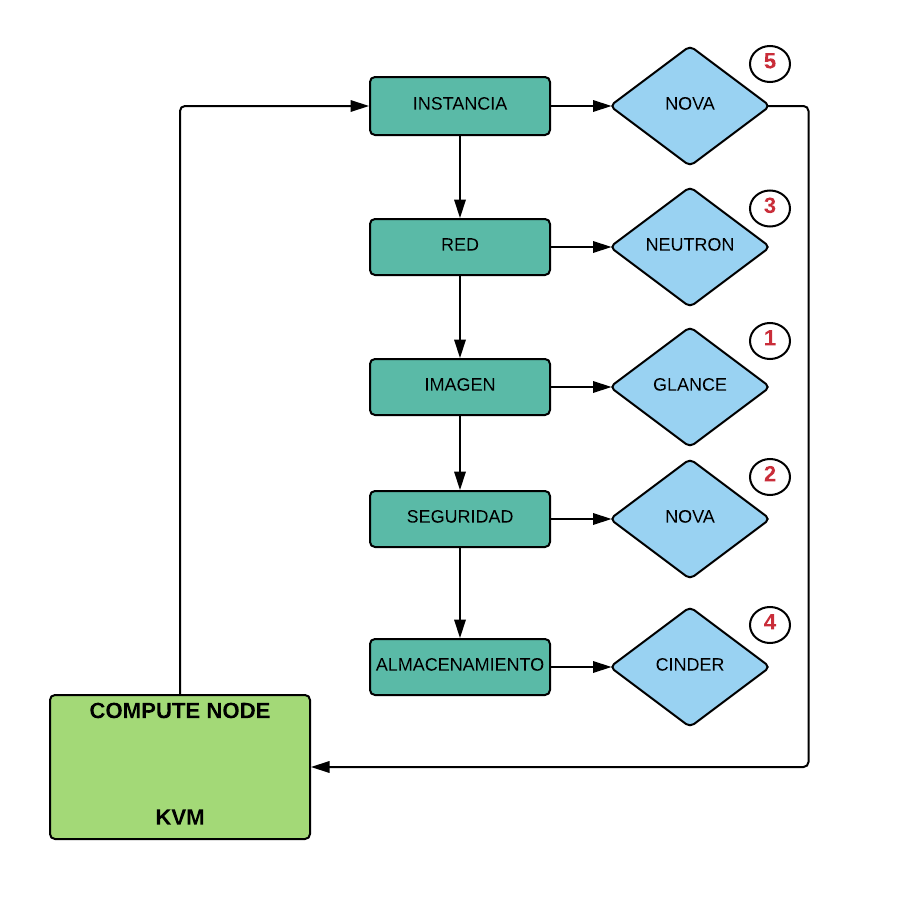
\includegraphics[width=0.7\textwidth]{imagenes/capitulo6/recursosInstancia.png}
    \caption{Recursos necesarios para la creación de una Instancia.}
	\vspace{0.3cm}
    \label{recursosInstancia}
\end{figure}

Así pues si queremos crear una instancia, no es tan simple como arrancarla sin más, necesitamos preparar otras elementos antes. En primer lugar la imagen en Glance que vamos a arrancar, un símil podría ser el ya nombrado de un live CD de Linux. Después, debemos asegurarnos de que en Nova tenemos configurada y activa la seguridad  pues de lo contrario no podremos acceder a la imagen. También tenemos que atender al networking y también al almacenamiento persistente si así lo queremos. Una vez realizadas estas tareas, podremos bootear desde Nova la instancia. Un esquema de los pasos podemos verlo en la Fig.\ref{recursosInstancia}.

De modo que los pasos a seguir son:

\begin{itemize}
\item Configurar la red
\item Asignar direcciones IP flotantes
\item Definir un grupo de seguridad en la nube
\item Crear un par de claves SSH
\item Crear una imagen de Glance
\item Eligir un \textit{flavor}, el cual contendrá las capacidades hardware reservadas para la instancia. 
\item Iniciar la instancia.
\end{itemize}

\subsection{IP flotante} \label{subsec:IP-flotante}
Las redes son una parte muy importante del entorno cloud. Antes incluso de comenzar a crear instancias en nuestra nube, como administradores de un tenant tendremos que crear el entorno de SDN. Esto implica que hemos de asegurarnos de que las instancias se puedan conectar a una red interna privada y también asignar direcciones IP flotantes para que puedan ser alcanzadas externamente.

En primer lugar vamos a definir el concepto de IP flotante en OpenStack. Una dirección IP flotante es un servicio proporcionado por Neutron. No se utiliza para la asignación ningún servicio DHCP ni está configurado de manera estática  dentro de la instancia o la máquina donde se ejecute. De hecho, el sistema operativo anfitrión no tiene idea de que se le asignó una dirección IP flotante. La entrega de paquetes a la interfaz con la dirección flotante asignada es responsabilidad del agente L3 de Neutron. 

A las instancias con una dirección IP flotante asignada se puede acceder desde la red pública mediante la IP flotante.
Una dirección IP flotante y una dirección IP privada se pueden usar al mismo tiempo en una única interfaz de red. Es probable que la dirección IP privada se use para la comunicación o acceso a otras instancias dentro de la red privada mientras que la dirección IP flotante se usará para acceder a la instancia desde redes públicas.

\begin{figure}
    \centering
    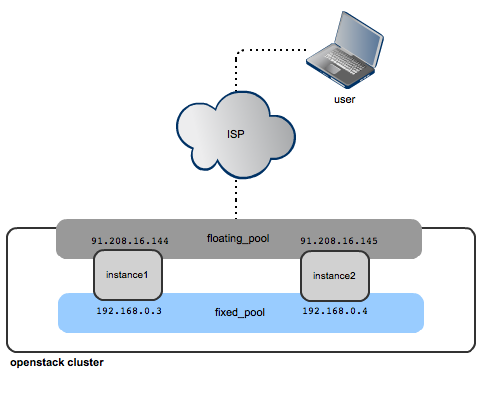
\includegraphics[width=0.7\textwidth]{imagenes/capitulo6/floatingIP.png}
    \caption{Esquema de uso de IPs flotantes.}
	\vspace{0.3cm}
    \footnotesize{Fuente: Mirantis }
    \label{ipsflotantes}
\end{figure}

Para explicar su funcionamiento pondremos un ejemplo de uso. En la Fig.\ref{ipsflotantes} podemos ver un diagrama que esquematiza un posible escenario donde se refleja el tema que estamos tratando. En la parte inferior de esta figura se puede ver que hay dos instancias: instancia 1 e instancia 2, y tienen direcciones IP que provienen de la red privada. La red privada es como una red detrás de un router NAT. Todo lo que está detrás del router NAT no se puede abordar directamente, por lo tanto, no se puede acceder a las direcciones IP 192.168.0.3 y 192.168.0.4 directamente desde Internet. Es por eso que en OpenStack, al crear nuestras SDN para hacer que las instancias sean accesibles, se necesitan direcciones IPs flotantes como se puede ver en la parte superior de la figura.\cite{noauthor_floating_2012}

Por tanto, una dirección IP flotante  es una dirección IP que está reservada para una instancia y está expuesta en el lado externo del router NAT. De este modo, para que el tráfico externo llegue a nuestra instancia creada, el tráfico externo deberá ir directamente a la dirección IP flotante de la instancia y es el router SDN el que se asegura de que todo el tráfico que llega, por ejemplo, a la IP 91.208.16.144, se reenvíe a la 192.168.0.2.

Hay una parte interesante en la configuración de todo esto y es que la dirección IP flotante no es conocida por la instancia como ya hemos comentado, sino que es conocida únicamente por el router SDN que la usa para llegar a la instancia. 

\subsection{Creación de redes}
Ya tenemos configurado un entorno de proyecto con un administrador de proyecto. El siguiente paso es comenzar a trabajar con instancias, Pero antes de que podamos comenzar a trabajar con instancias debemos encargarnos de definir las redes.

Desde dentro de Horizon, en el apartado  “Proyecto-\textgreater Red-\textgreater Redes”, el primer paso será crear una nueva red definida por software. Para hacerlo, hacemos clic en “Crear red” y la le ponemos el nombre “horizon-private-net” %(Fig.\ref{crearRed})
. Esta será nuestra red privada o interna.

\begin{tcolorbox}[colback=green!5!white,colframe=green!75!black]
FALTA FIGURA....................................................

....................................................FALTA FIGURA
\end{tcolorbox}

\begin{comment}
\begin{figure}
    \centering
    \includegraphics[width=0.7\textwidth]{imagenes/capitulo6/crearRed.PNG}
    \caption{Creando una red desde Horizon.}
	\vspace{0.3cm}
    \label{crearRed}
\end{figure}
\end{comment}

Al configurar una SDN, es muy importante hacer una distinción entre la red interna y la red externa. La red interna es a la que se conectarán las máquinas virtuales  que creemos mientras que la red externa es la que nos permitirá conectarnos con nuestra infraestructura de red física.

El siguiente paso es crear una subred desde la pestaña de la misma ventana “Subred”. Vamos a llamarla “horizon-private-subnet”. Esta subred necesita una dirección de red, usaremos 192.170.1.0/24 %como vemos en la Fig.\ref{crearSubRed}. 
Se puede usar cualquier dirección IP que deseemos siempre que sea una dirección IP privada. Esta es la subred que usarán internamente solo las máquinas virtuales y permitirá que las máquinas virtuales en la nube se comuniquen entre sí.

\begin{tcolorbox}[colback=green!5!white,colframe=green!75!black]
FALTA FIGURA....................................................

....................................................FALTA FIGURA
\end{tcolorbox}

\begin{comment}
\begin{figure}
    \centering
    \includegraphics[width=0.7\textwidth]{imagenes/capitulo6/crearSubRed.PNG}
    \caption{Creando una subred desde Horizon.}
	\vspace{0.3cm}
    \label{crearSubRed}
\end{figure}
\end{comment}

En nuestro rango de red IP, es probable que deseemos tener una puerta de enlace o \textit{gateway} también. Podemos especificar la puerta de enlace, pero si no lo hacemos, obtendremos una dirección de puerta de enlace predeterminada, ya que en cualquier red para que las máquinas se comuniquen con el mundo exterior, necesitamos pasarelas en todo momento. En caso de que no queramos una puerta de enlace, podemos hacer clic específicamente en “Deshabilitar puerta de enlace”, pero eso normalmente no es algo que deseemos hacer.

En  la siguiente pestaña tenemos el bloque de  “Detalles de Subred”. En los detalles de la subred podemos especificar el resto de elementos necesarios para especificar nuestra subred. Básicamente esto se reduce a la configuración de DHCP. DHCP se asegurará de que nuestras instancias obtengan una dirección IP por defecto en el rango de subred especificado. En el campo “Pools de asignación”, necesitamos crear una lista de direcciones IP separada por comas con la primera dirección en el grupo de asignación y la última dirección en el grupo de asignación, o una dirección por línea si así lo queremos. En este caso, crearemos un rango de direcciones DHCP válidas dentro de la subred que irá desde la 192.170.1.100 a la 192.170.1.150. %Como evidencia mostramos la Fig.\ref{crearSubRedDetails}.

\begin{tcolorbox}[colback=green!5!white,colframe=green!75!black]
FALTA FIGURA....................................................

....................................................FALTA FIGURA
\end{tcolorbox}

\begin{comment}
\begin{figure}
    \centering
    \includegraphics[width=0.7\textwidth]{imagenes/capitulo6/crearSubRedDetails.PNG}
    \caption{Configuración de DHCP y DNS.}
	\vspace{0.3cm}
    \label{crearSubRedDetails}
\end{figure}
\end{comment}

También podemos especificar el o los servidores DNS en el campo “Servidores DNS”, asignando así un servidor de nombres a las instancias y también podemos crear rutas a host específicos en el campo “Rutas de host”. Normalmente, esto no será necesario ya que la gateway creada por defecto se encargará de ello. Haciendo clic en “Crear” tendremos la red a punto.

En este punto, debemos asegurarnos de que haya también una red pública. La red pública podríamos crearla de forma análoga clicando de nuevo en “Crear red” y habilitándola como red pública después desde el tenant de administrador, pero está red ya se creo en la instalación inicial de manera automática en base a los parámetros de configuración introducidos en el archivo \textit{local.conf} (ver apéndice \ref{chap:manualdeinstalacion}).

Una vez tenemos ambas redes podremos ver que aparecen en nuestro panel.

\begin{tcolorbox}[colback=green!5!white,colframe=green!75!black]
FALTA FIGURA....................................................

....................................................FALTA FIGURA
\end{tcolorbox}

\begin{comment}
\begin{figure}
    \centering
    \includegraphics[width=0.7\textwidth]{imagenes/capitulo6/redesCreadas.PNG}
    \caption{Panel de red.}
	\vspace{0.3cm}
    \label{redesCreadas}
\end{figure}
\end{comment}

\subsection{Creación de routers}
El siguiente paso será establecer una conexión entre la red pública y la red privada para lo cual necesitaremos crear un router. En la pestaña “Proyecto-\textgreater Red-\textgreater Routers” cliclamos en “Crear Router” y nombramos el router a crear como “horizon-router”. 

Además tendremos que seleccionar una red externa que será la red pública creada nombrada como “public”. Haciendo clic en “Crear Router” tendremos el router creado y en la topología de red que vemos en la %Fig.\ref{crearRouter}
aparecerá conectado a la red pública. Si pasamos el cursor sobre el icono “horizon-router”, podemos ver diferentes opciones. De ellas seleccionamos “Añadir interfaz” para agregar una  nueva interfaz que nos permitirá conectar nuestro router también con la red interna “horizon-private-net”, al seleccionarla, automáticamente conecta el router con esa red creando una interfaz que tiene asignada la dirección IP 192.170.1.1, dentro del rango de direcciones de la subred que creamos.

\begin{tcolorbox}[colback=green!5!white,colframe=green!75!black]
FALTA FIGURA....................................................

....................................................FALTA FIGURA
\end{tcolorbox}
\begin{comment}

\begin{figure}
    \centering
    \includegraphics[width=0.7\textwidth]{imagenes/capitulo6/crearRouter.PNG}
    \caption{Creación de un router.}
	\vspace{0.3cm}
    \label{crearRouter}
\end{figure}
\end{comment}


\begin{tcolorbox}[colback=green!5!white,colframe=green!75!black]
FALTA FIGURA....................................................

....................................................FALTA FIGURA
\end{tcolorbox}

\begin{comment}
\begin{figure}
    \centering
    \includegraphics[width=0.7\textwidth]{imagenes/capitulo6/addInterfazRouter.PNG}
    \caption{Añadir interfaz a un router.}
	\vspace{0.3cm}
    \label{addInterfazRouter}
\end{figure}
\end{comment}


\subsection{Implementar una instancia desde Horizon}
Ahora que se ha configurado la red, podemos encargarnos del resto. Para empezar, tendremos que crear un grupo de seguridad o \textit{security group}. El grupo de seguridad es un conjunto de reglas de firewall que se aplicarán desde la nube a una instancia. La idea es que la instancia se genere desde una imagen de Glance. En una imagen de Glance, no se pueden definir las reglas de firewall que deben aplicarse y es por eso que tenemos que definirlas a través de la creación de un grupo de seguridad en la nube.

El siguiente paso por tanto es crear un par de claves SSH (\textit{SSH Key Pair}). SSH key pair consiste en un conjunto de clave pública-privada. La clave privada se mantiene en la estación de trabajo y la clave pública en la instancia, por tanto, el par de claves SSH nos sirve para permitir una conexión segura a la instancia. La otra opción sería acceder a la instancia utilizando contraseñas predeterminadas y nombres de usuario predeterminados lo cual es muy inseguro por lo que utilizando SSH Key Pairs, aumentamos el nivel de seguridad. Estas claves generadas serán las que usemos más tarde para conectarnos a las instancias creadas a través de un terminal.

También necesitamos la imagen de Glance. Una imagen de Glance es como un live CD de Linux. Veremos cómo podemos descargar una imagen usando de Cirros desde la nube.

Por último tenemos el flavor que también tendremos que seleccionar. Un flavor es básicamente el perfil de hardware que elegiremos para nuestra instancia. De este modo, si creamos una instancia de una imagen de Glance, determinaremos cuánta RAM, cuánto espacio en disco, etc., va a usar dicha instancia. Una vez que hayamos seguido este proceso, podremos arrancar la instancia.


En este punto, tenemos una red operativa, lo cual significa que cumplimos con todos los requisitos para implementar instancias desde Horizon. En primer lugar, tendremos que entrar en Horizon como tenant “horizon-user”, un usuario cualquiera, ya que el administrador de la nube no va a derivar instancias para los inquilinos si no que lo harán ellos mismos.

\subsection{Creación de grupos de seguridad}
Lo primero que vamos a crear es un grupo de seguridad. Un grupo de seguridad es un firewall. La razón por la que estamos trabajando con grupos de seguridad en entornos de nube es que, si se derivan las instancias de la nube de forma dinámica, no es posible crear firewalls diferenciados dentro de las instancias de la nube, y es por eso que vamos a definir el firewall desde la nube y asignarlo a las instancias. Para hacerlo, dentro de “Red”, en el apartado de “Grupos de seguridad”. Le daremos el nombre de “horizon-secgroup” tal como vemos en la %Fig.\ref{createSecGroup}

\begin{tcolorbox}[colback=green!5!white,colframe=green!75!black]
FALTA FIGURA....................................................

....................................................FALTA FIGURA
\end{tcolorbox}

\begin{comment}
\begin{figure}
    \centering
    \includegraphics[width=0.7\textwidth]{imagenes/capitulo6/createSecGroup.PNG}
    \caption{Creación de un grupo de seguridad.}
	\vspace{0.3cm}
    \label{createSecGroup}
\end{figure}
\end{comment}

Una vez creado haciendo clic en el “Administar reglas” del campo “Acciones” del grupo de seguridad creado vamos a definir algunas reglas de seguridad. Las reglas de seguridad funcionan de manera similar a como se hacen creando listas de acceso en un router de Cisco por ejemplo. Por defecto, tal como aparece en la %Fig.\ref{crearReglas}
, tenemos permitido tráfico saliente permitido en IPv4 a cualquier parte, y tenemos tráfico saliente permitido en IPv6 en cualquier lugar, además, de manera predeterminada el tráfico entrante no está permitido.

\begin{tcolorbox}[colback=green!5!white,colframe=green!75!black]
FALTA FIGURA....................................................

....................................................FALTA FIGURA
\end{tcolorbox}

\begin{comment}
\begin{figure}
    \centering
    \includegraphics[width=0.7\textwidth]{imagenes/capitulo6/crearReglas.PNG}
    \caption{Reglas por defecto y creación de nuevas reglas.}
	\vspace{0.3cm}
    \label{crearReglas}
\end{figure}
\end{comment}


Podemos crear reglas nuevas pulsando en “Agregar regla”. En primer lugar agregaremos una regla del tipo “Todos los ICMP” cuyos parámetros vemos en la %Fig.\ref{reglaICMP}
. Esta regla especificamos en el campo “Dirección”, “Entrante”, para indicar que se trata de una regla acerca del tráfico ICMP de entrada, en el campo “Remoto” seleccionamos “CIDR” y como CIDR (\textit{Classless Inter-Domain Routing}) 0.0.0.0/0, indicando así que permitimos cualquier dirección IP, permitiendo de este modo que las instancias creadas puedan ser alcanzadas por cualquiera.

\begin{tcolorbox}[colback=green!5!white,colframe=green!75!black]
FALTA FIGURA....................................................

....................................................FALTA FIGURA
\end{tcolorbox}

\begin{comment}
\begin{figure}
    \centering
    \includegraphics[width=0.7\textwidth]{imagenes/capitulo6/reglaICMP.PNG}
    \caption{Creación de una regla para el tráfico ICMP.}
	\vspace{0.3cm}
    \label{reglaICMP}
\end{figure}
\end{comment}

Creamos una regla más del mismo modo. Esta vez vamos a permitir el tráfico HTTP para lo que en “Regla” marcamos “HTTP” con “CIDR”, 0.0.0.0/0, y una última, sobre el tráfico SSH con los mismos parámetros, la cual es de vital importancia ya que a las instancias, de manera predeterminada, accederemos como usuarios vía SSH y tenemos que permitirlo en el firewall. Una creadas todas se mostrarán en el panel como se aprecia en la %Fig.\ref{reglasCreadas}.

\begin{comment}
\begin{figure}
    \centering
    \includegraphics[width=0.7\textwidth]{imagenes/capitulo6/reglasCreadas.PNG}
    \caption{Panel de grupos de seguridad con las reglas creadas.}
	\vspace{0.3cm}
    \label{reglasCreadas}
\end{figure}
\end{comment}

\subsection{Creación de IPs flotantes}
En el siguiente paso trabajaremos con direcciones IP flotantes. Una dirección IP flotante es una dirección IP que se utilizará para hacer que la instancia sea accesible desde el exterior. La razón por la que las necesitamos es que por defecto, las instancias son visibles sólo en la red privada. Si solo están en la red privada, nadie externo podrá acceder a ellas, y es por eso que debemos usar direcciones IP flotantes.

Por tanto, una dirección IP flotante es una dirección IP en la nube, y todo lo que entra en la dirección IP flotante se reenviará a la dirección IP de la instancia. Esto significa que la dirección IP flotante debe estar disponible en la red externa, que es la red pública que creamos como “public”, lo que implica que debemos asegurarnos de que cuando se está construyendo la nube, la red pública tenga una cantidad significativa de direcciones IP disponibles. Por esto motivo, en la preparación de los servidores creamos una interfaz virtual de la tarjeta de red disponible, ya que al sólo tener una, sólo podíamos disponer de una dirección IP flotante. De este modo conseguimos tener un pool de direcciones IPs flotantes disponibles para asignar a las instancias.

Comenzamos moviéndonos al apartado “Proyecto-\textgreater Red-\textgreater IPs flotantes” y clicamos en “Asignar IP al proyecto” para asignar una IP flotante al proyecto, que se creará automáticamente del pool que habíamos creado como vemos en la %Fig\ref{crearIPflotante}
. Necesitaremos una IP flotante por cada instancia que creemos, luego siguiendo el mismo proceso podemos crear tantas como nuestra quota nos permita. 

\begin{tcolorbox}[colback=green!5!white,colframe=green!75!black]
FALTA FIGURA....................................................

....................................................FALTA FIGURA
\end{tcolorbox}

\begin{comment}
\begin{figure}
    \centering
    \includegraphics[width=0.7\textwidth]{imagenes/capitulo6/crearIPflotante.PNG}
    \caption{Creación de una IP flotante.}
	\vspace{0.3cm}
    \label{crearIPflotante}
\end{figure}
\end{comment}

\subsection{Creación de pares de claves público-privada}
Para llegar al paso de la %Fig.\ref{horizon-keypair} 
iremos ahora al apartado  “Proyecto-\textgreater Compute”, donde vamos a encargarnos  de las instancias. Antes de que podamos derivar una instancia, necesitamos un par de claves SSH, por tanto en primer lugar clicamos en “Pares de claves” y dentro del apartado “Crear Par de de Claves”. Tenemos que darle un nombre que será “horizon-keypair” y pulsar en “Crear Par de Claves” para que se genere

\begin{tcolorbox}[colback=green!5!white,colframe=green!75!black]
FALTA FIGURA....................................................

....................................................FALTA FIGURA
\end{tcolorbox}


\begin{comment}
\begin{figure}
    \centering
    \includegraphics[width=0.7\textwidth]{imagenes/capitulo6/horizon-keypair.PNG}
    \caption{Creación de un par de claves.}
	\vspace{0.3cm}
    \label{horizon-keypair}
\end{figure}
\end{comment}

Una vez creada podremos descargarla para usarla después. Esta clave privada es una clave que debe estar disponible y por tanto almacenada en la estación de trabajo del usuario final.

Si nos encontramos en el PC que vaya a hacer de estación de trabajo, en mi caso mi ordenador personal, vamos al directorio “.ssh” y copiaremos la clave privada generada para alojarla en la estación de trabajo:

\begin{lstlisting}[style=Consola]
atj@wimunet4:~/devstack$$ ls -l | grep key
-rw-rw-r-- 1 atj atj 1679 sep  6 10:52 horizon-keypair
atj@wimunet4:~/devstack$ chmod 400 horizon-keypair
atj@wimunet4:~/devstack$ ls -l | grep MyKeyP
-r-------- 1 atj atj 1679 sep  6 10:52 horizon-keypair
atj@wimunet4:~/devstack$ cp horizon-keypair /home/atj/.ssh
\end{lstlisting}

“ls -l” muestra los permisos que necesitamos. Esta clave privada será utilizada por el usuario final para conectar a los servidores que tienen una copia de la clave pública disponible, necesario para entrar a las instancias que se implementarán en OpenStack. También hemos cambiado el tipo de permisos ya que inicialmente no era el correcto. La clave privada debe ser altamente segura, por lo que es aconsejable cambiarle los permisos.

\subsection{Creación de imágenes}
El siguiente paso está encaminado a la creación de imágenes. Necesitamos las imágenes porque las instancias de la nube de OpenStack no están instaladas, sino que se implementan. La instalación funciona para un centro de datos tradicional, donde un administrador pasa por todas las diferentes opciones para instalar una máquina virtual. Eso no es lo que se hace en OpenStack. En OpenStack, la implementamos utilizando una imagen lista para ser usada.

En nuestro caso vamos a usar la imagen de Cirros, que es más ligera y por motivos de capacidad la más aconsejable. Antes de poder usarla necesitamos realizar la descarga de la imagen desde la máquina en la que se esté ejecutando Horizon, en nuestro caso nuestro servidor. Para iniciar la descarga en caso de que no hubiesemos incorporado la misma en el script de configuración incial o quisieramos otra podemos escribir desde una consola dentro de la máquina que aloja OpenStack:
% o ponerla en el script de configuración

\begin{lstlisting}[style=Consola]
stack@wimunet4:~/devstack$ wget http://download.cirros-cloud.net/0.4.0/cirros-0.4.0-x86_64-disk.img
\end{lstlisting}

Cirros es una imagen de nube que nos permitirá probar la implementación de instancias en una nube de OpenStack o en cualquier otra nube. Esta imagen no sería la que usaríamos en un entorno cloud de producción, pero es altamente aconsejable para nuestro propósito debido a que las imágenes de cirros son realmente pequeñas, por lo que no supondrá una gran capacidad de los recursos que tenemos disponibles en nuestra máquina. Por supuesto, existen también otras imágenes en la nube disponibles \cite{noauthor_openstack_nodate-7}, pero estas requieren más requisitos hardware y suelen modificarse para usarse en entornos de producción.

Una vez que tenemos la imagen en la nube disponible, podemos volver a Horizon para crear nuestra imagen con los parámetros de la %Fig.\ref{crearImagenHorizon}
, y dentro de  “Proyecto-\textgreater Compute-\textgreater Imágenes” hacer clic en “Crear imagen”. Vamos a llamar “horizon-cirros” y especificamos el tipo de formato, que será QCOW2. QCOW2 es un formato de imagen de nube común, tenemos otros formatos disponibles, también, pero de nuevo no es recomendable usar ninguno de ellos ya que son para entornos específicos que no deseamos usar por el momento. Tenemos una opción en el campo “Compartir imagen” interesante, ya que permite establecer una imagen como protegida o no. Puesto que es una imagen que como usuario tenant, queremos que esté disponible para todos los demás, marcaremos la opción “No”. Después de hacerlo, haciendo clic en “Create Image” importaremos la imagen a nuestro entorno de nube OpenStack. 

\begin{tcolorbox}[colback=green!5!white,colframe=green!75!black]
FALTA FIGURA....................................................

....................................................FALTA FIGURA
\end{tcolorbox}


\begin{comment}
\begin{figure}
    \centering
    \includegraphics[width=0.7\textwidth]{imagenes/capitulo6/crearImagenHorizon.PNG}
    \caption{Creación de una imagen: Detalles.}
	\vspace{0.3cm}
    \label{crearImagenHorizon}
\end{figure}
\end{comment}

\subsection{Creación de instancias}
Una vez que la imagen se ha importado con éxito, vamos a “Proyecto-\textgreater Compute-\textgreater Instancias” y seleccionamos “Lanzar instancia”. Esto nos lleva a una lista de diferentes items que podemos configurar al iniciar una instancia. Todo lo que está marcado con un asterisco es obligatorio y el resto opcional como podemos ver en la %Fig.\ref{creandoInstancia}
, donde en primer lugar le damos un nombre a la instancia, “horizon-instance-1”. La opción “Count” permite lanzar más instancias al mismo tiempo. Haciendo clic en “Siguiente” pasaremos a especificar el origen de arranque, que será nuestra imagen importada, además podemos decidir si crear un volumén que se asiganará a esa instancia y si tras eliminar la misma mantendremos el volumen o no quedando así la configuración de la %Fig.\ref{origenInstancia}
.

\begin{tcolorbox}[colback=green!5!white,colframe=green!75!black]
FALTA FIGURA....................................................

....................................................FALTA FIGURA
\end{tcolorbox}


\begin{comment}
\begin{figure}
    \centering
    \includegraphics[width=0.7\textwidth]{imagenes/capitulo6/origenInstancia.PNG}
    \caption{Creación de una imagen: Origen.}
	\vspace{0.3cm}
    \label{origenInstancia}
\end{figure}
\end{comment}


Pulsamos “Siguiente” y seleccionamos el “Sabor” (del ingés \textit{flavor}) para especificar el perfil de hardware que va a utilizar nuestra instancia. Podríamos crear nuestros propios flavors si así lo queremos, de hecho, para tener un flavor que se ajuste más a los requisitos que necesite nuestra máquina vamos a crear el que usaremos a continuación del siguiente modo:

\begin{lstlisting}[style=Consola]
stack@wimunet4:~/devstack$ source openrc admin admin
stack@wimunet4:~/devstack$ openstack flavor create --ram 512 --disk 4 --vcpus 1 m1.little
\end{lstlisting}

El motivo de autenticarnos antes como usuario administrador del entorno, es que este flavor pueda estar disponible para cualquier usuario ya que si lo hacemos desde un tenant específico, como por ejemplo el que estamos usando, horizon-user, sólo estaría disponible para el projecto horizon-project. De acuerdo a la configuración introducida, la imagen que asociemos a este flavor de acuerdo al orden de parámetros introducido tendrá una RAM de 512 MB, 4 GB de disco reservada para la partición /root, una única CPU virtual y como nombre \textit{m1.little}. De igual modo podríamos haberlo hecho desde horizon autenticándonos como admin dentro del apartado “Proyecto-\textgreater Compute-\textgreater Instancias-\textgreater Crear Sabor”. 

Una vez creado, podemos continuar con la creación de la instancia y seleccionarlo dentro de las opciones disponibles en el apartado flavor %(Fig.\ref{flavorInstance})
.

\begin{tcolorbox}[colback=green!5!white,colframe=green!75!black]
FALTA FIGURA....................................................

....................................................FALTA FIGURA
\end{tcolorbox}


\begin{comment}
\begin{figure}
    \centering
    \includegraphics[width=0.7\textwidth]{imagenes/capitulo6/flavorInstance.PNG}
    \caption{Creación de una imagen: Sabor.}
	\vspace{0.3cm}
    \label{flavorInstance}
\end{figure}
\end{comment}

Con esta configuración ya podríamos crear la instancia pero vamos a especificar algunos parámetros de configuración más. Ahora, como vemos en la %Fig.\ref{redesInstancia}
iremos al apartado “Redes” dentro de las opciones de creación de la instancia veremos las redes que se han creado. Necesitamos que esté disponible en “horizon-private-net” para asignar las instancias que creamos a la red interna y luego hacerlas accesibles a través de una dirección IP flotante. 

\begin{tcolorbox}[colback=green!5!white,colframe=green!75!black]
FALTA FIGURA....................................................

....................................................FALTA FIGURA
\end{tcolorbox}


\begin{comment}
\begin{figure}
    \centering
    \includegraphics[width=0.7\textwidth]{imagenes/capitulo6/redesInstancia.PNG}
    \caption{Creación de una imagen: Redes.}
	\vspace{0.3cm}
    \label{redesInstancia}
\end{figure}
\end{comment}


No necesitamos asignar puertos por lo que pasamos a “Grupos de Seguridad”. Es imporante asignarle el grupo creado, pues de lo contrario tendremos una instancia que no será accesible en absoluto. Hacemos clic en la flecha hacia arriba para asignar el grupo “horizon-secgroup” que aparece en la %Fig\ref{secgroupInstancia}
como grupo de seguridad a la instancia. 

\begin{tcolorbox}[colback=green!5!white,colframe=green!75!black]
FALTA FIGURA....................................................

....................................................FALTA FIGURA
\end{tcolorbox}


\begin{comment}
\begin{figure}
    \centering
    \includegraphics[width=0.7\textwidth]{imagenes/capitulo6/secgroupInstancia.PNG}
    \caption{Creación de una imagen: Grupos de Seguridad.}
	\vspace{0.3cm}
    \label{secgroupInstancia}
\end{figure}
\end{comment}


Finalmente en el apartado “Pares de Claves” elegimos “horizon-keypair” y ya podremos cargar la instancia pulsando en el botón “Ejecutar Instancia” de la %Fig.\ref{keyInstancia}
.


\begin{tcolorbox}[colback=green!5!white,colframe=green!75!black]
FALTA FIGURA....................................................

....................................................FALTA FIGURA
\end{tcolorbox}


\begin{comment}
\begin{figure}
    \centering
    \includegraphics[width=0.7\textwidth]{imagenes/capitulo6/keyInstancia.PNG}
    \caption{Creación de una imagen: Par de Claves.}
	\vspace{0.3cm}
    \label{keyInstancia}
\end{figure}
\end{comment}


\subsection{Creación de volúmenes de almacenamiento para las instancias}
\begin{tcolorbox}[colback=red!5!red,colframe=red!75!black]
Quitar la parte de creación de un volumen anterior y meterla aquí.
\end{tcolorbox}



%“”
%“”
%“”
%“”
\section{Configuración de un escenario mediante la CLI}
En este apartado vamos a ver como se puede crear también un escenario como en el caso anterior, pero esta vez desde línea de comandos. Puesto que hemos ido explicando y motivando cada paso en el apartado anterior, vamos a ir directos aquí a las pasos a seguir para alcanzar nuestro objetivo, listando los comandos necesarios para la consecución del acceso a las instancias.

La lista de comandos de OpenStack para administrar la CLI se puede consultar en la documentación pertinente.\cite{noauthor_command_nodate}

Para automatizar el proceso que aquí veremos y ver así la evolución en la administración de OpenStack de la que hablábamos en la sección \ref{subchap:heat} hemos creado un script en bash con el nombre \textit{cli\_creacion\_escenario.sh}. Este script podremos verlo en el apéndice \ref{chap:creacionescenariobash}.

\subsection{Credenciales}
Lo primero que debemos hacer al acceder a la CLI, es autenticarnos con las credenciales de OpenStack de aquel usuario con el que queramos acceder a nuestro entorno. Cuando creamos un usuario, Keystone almacena en su base de datos las credenciales del mismo. Para acceder a ellas y autenticarnos, en este caso como usuario administrados, se indica el nombre del proyecto y el usuario que tenemos:

\begin{lstlisting}[style=Consola]
stack@wimunet4:~/devstack$ source openrc admin admin
\end{lstlisting}

Para establecer las variables de entorno requeridas para los clientes desde la CLI de OpenStack, se debe crear un archivo de entorno llamado archivo \textit{openrc.sh} que en nuestro caso se proporciona al instalar DevStack. Este archivo de entorno específico del proyecto contiene las credenciales que utilizan todos los servicios de OpenStack. De este modo, las variables de entorno se establecen para nuestro \textit{shell} actual. Las variables permiten que los comandos del cliente OpenStack se comuniquen con los servicios OpenStack que se ejecutan en la nube.\cite{noauthor_openrc_nodate}

\subsection{Creación de proyectos o tenants}
\begin{lstlisting}[style=Consola]
stack@wimunet4:~/devstack$ openstack project create --description 'Escenario creado con cli' cli-project --domain default
\end{lstlisting}

\begin{lstlisting}[style=Consola]
stack@wimunet4:~/devstack$ openstack quota set cli-project --instances 10
stack@wimunet4:~/devstack$ openstack quota set cli-project --ram 4096 
\end{lstlisting}

\subsection{Creación de usuarios}
\begin{lstlisting}[style=Consola]
stack@wimunet4:~/devstack$ openstack user create --project cli-project --password temporary cli-user
\end{lstlisting}

\begin{lstlisting}[style=Consola]
stack@wimunet4:~/devstack$ openstack role add --user cli-user --project cli-project Member
\end{lstlisting}

\subsection{Creación de redes}
Vamos a ver en este apartado como crear elementos de conectividad de red, en concreto redes y subredes desde la CLI.

Para crear una red escribimos el siguiente comando:

\begin{lstlisting}[style=Consola]
stack@wimunet4:~/devstack$ openstack network create cli-private-net 
\end{lstlisting}

Se nos devolverá:

\begin{tcolorbox}[colback=green!5!white,colframe=green!75!black]
FALTA FIGURA....................................................

....................................................FALTA FIGURA
\end{tcolorbox}

De este modo crearemos una red llamada \textit{cli-private-net}. No necesitamos propiedades adicionales puesto que estas se declaran en la subred. Así pues este será el siguiente paso:

\begin{lstlisting}[style=Consola]
stack@wimunet4:~/devstack$ openstack subnet create --network cli-private-net --subnet-range 192.168.20.0/24 cli-private-subnet
\end{lstlisting}

Donde los parámetros que aparecen indican:
\begin{itemize}
\item --network cli-private-net. La red a la que queremos asociar la subred.
\item --subnet-range 192.168.20.0/24. El rango de la subred.
\item cli-private-subnet. Nombre que le hemos dado a la subred.
\end{itemize}

Con esto se nos devolverán los parámetros para la subred creada:

\begin{tcolorbox}[colback=green!5!white,colframe=green!75!black]
FALTA FIGURA....................................................

....................................................FALTA FIGURA
\end{tcolorbox}

\subsection{Creación de routers}
Para hacer las redes creadas accesibles necesitamos crear un router.

\begin{lstlisting}[style=Consola]
stack@wimunet4:~/devstack$ openstack router create cli-router
\end{lstlisting}

Para tener acceso a la subred \textit{cli-private-subnet} necesitamos conectar el router creado a esta subred.

\begin{lstlisting}[style=Consola]
stack@wimunet4:~/devstack$ openstack router add subnet cli-router cli-private-subnet
\end{lstlisting}

Y también a la red pública que ya teníamos creada cuyo nombre es \textit{public} con el siguiente comando y el parámetro --external-gateway para indicar que se trata de la puerta de enlace a la red externa.

\begin{lstlisting}[style=Consola]
stack@wimunet4:~/devstack$ openstack router set cli-router --external-gateway public
\end{lstlisting}

Podemos una vez realizada la configuración de los parámetros de red ver como queda la configuración del router como se ve en la Fig. mediante el siguiente comando:

\begin{lstlisting}[style=Consola]
stack@wimunet4:~/devstack$ openstack show cli-router
\end{lstlisting}

\begin{tcolorbox}[colback=green!5!white,colframe=green!75!black]
FALTA FIGURA....................................................

....................................................FALTA FIGURA
\end{tcolorbox}

\subsection{Creación de grupos de seguridad}
Ahora vamos a ver como crear un grupo de seguridad que como sabemos hará las veces de firewall para las instancias:

\begin{lstlisting}[style=Consola]
stack@wimunet4:~/devstack$ openstack security group create cli-secgroup
\end{lstlisting}

Con esto habremos creado un grupo de seguridad llamado \textit{cli-secgroup}. Para que actúe como nosotros queremos, crearemos una serie de reglas que permitan el tráfico que deseamos y el resto no. Por defecto, todo el tráfico saliente esta permitido. Para el entrante:

\begin{lstlisting}[style=Consola]
stack@wimunet4:~/devstack$ openstack  security group rule create --remote-ip 0.0.0.0/0 --protocol tcp --dst-port 22  --ingress cli-secgroup
stack@wimunet4:~/devstack$ openstack  security group rule create --remote-ip 0.0.0.0/0 --protocol icmp --ingress cli-secgroup
stack@wimunet4:~/devstack$ openstack  security group rule create --remote-ip 0.0.0.0/0 --protocol tcp --dst-port 80:80  --ingress cli-secgroup
\end{lstlisting}

Donde hemos creado tres reglas de seguridad asignadas al grupo de seguridad \textit{cli-group} que permiten en tráfico ICMP, SSH y HTTP desde cualquier dirección.

Podemos consultar si las reglas del grupo se han creado con éxito escribiendo:

\begin{lstlisting}[style=Consola]
stack@wimunet4:~/devstack$ openstack security group show cli-secgroup
\end{lstlisting}

Que nos devolverá:

\begin{tcolorbox}[colback=green!5!white,colframe=green!75!black]
FALTA FIGURA....................................................

....................................................FALTA FIGURA
\end{tcolorbox}




\subsection{Creación de IPs flotantes}
Necesitamos también crear IPs flotantes para poder acceder remotamente a las instancias.

\begin{lstlisting}[style=Consola]
stack@wimunet4:~/devstack$ openstack floating ip create public
\end{lstlisting}

Y nos devolverá la IP flotante creada.

\begin{tcolorbox}[colback=green!5!white,colframe=green!75!black]
FALTA FIGURA....................................................

....................................................FALTA FIGURA
\end{tcolorbox}

Este paso lo repetiremos las veces que sea necesaria, tantas como IPs flotantes necesitemos. Un listado de todas las IPs flotantes que tenemos podemos obtenerlo escribiendo en la CLI:

\begin{lstlisting}[style=Consola]
stack@wimunet4:~/devstack$ openstack floating ip list
\end{lstlisting}

Que nos devolverá la lista de IPs flotantes disponibles.

\begin{tcolorbox}[colback=green!5!white,colframe=green!75!black]
FALTA FIGURA....................................................

....................................................FALTA FIGURA
\end{tcolorbox}

\subsection{Creación de pares de claves público-privada}
Vamos a crear ahora una clave para el acceso a las instancias vía SSH que llamaremos \textit{cli-keypair} y guardaremos como \textit{cli-keypair.pem} para su posterior uso cuando queramos acceder a las instancias a las que se les haya asignado esa clave:

\begin{lstlisting}[style=Consola]
stack@wimunet4:~/devstack$ openstack keypair create cli-keypair > cli-keypair.pem
stack@wimunet4:~/devstack$ chmod 0600 cli-keypair.pem
stack@wimunet4:~/devstack$ ssh-add cli-keypair.pem
\end{lstlisting}

Además como vemos hemos modificado los permisos de la clave creada para que sea más segura, pues no es algo a lo que queramos que todos los usuarios tengan acceso, y la hemos añadido a la lista de claves ssh.

Para comprobar que se ha creado correctamente podemos escribir:
\begin{lstlisting}[style=Consola]
stack@wimunet4:~/devstack$ openstack keypair list
\end{lstlisting}

Y veremos (Fig.) como aparece disponible con su correspondiente huella digital o \textit{fingerprint}.


\subsection{Creación de imágenes}
% como user
Almacenaremos todas la imágenes que queramos descargar en la carpeta \textit{images} creada para tal fin:

\begin{lstlisting}[style=Consola]
stack@wimunet4:~/devstack$ mkdir image
\end{lstlisting}

Para preparar la imagen de Cirros la descargamos del repositorio de imágenes de OpenStack:

\begin{lstlisting}[style=Consola]
stack@wimunet4:~/devstack$ wget https://download.cirros-cloud.net/0.4.0/cirros-0.4.0-x86_64-disk.img
\end{lstlisting}

Aunque no es estrictamente necesario al no ser que obtenemos por la descarga de otra imagen puesto que en el archivo de configuración \textit{local.conf} que recordemos podemos ver en el apéndice \ref{chap:manualdeinstalacion} ya impusimos la descarga automática de la misma.

Para crear la imagen escribimos:

\begin{lstlisting}[style=Consola]
stack@wimunet4:~/devstack$ openstack image create --disk-format qcow2 --min-disk 2 --file /opt/stack/devstack/images/cirros-0.4.0-x86_64-disk.img  --private cli-cirros
\end{lstlisting}

Con estemos comando estamos indicando que queremos crear una imagen de las siguientes características:
\begin{itemize}
\item --disk-format. Formato \textit{qcow2} que es el predeterminado para los entornos cloud.
\item --min-disk 2. Creando así un disco de al menos 2 GB.
\item --file /opt/stack/devstack/images/cirros-0.4.0-x86\_64-disk.img. Para indicar la ruta en la que se encuentra la imagen de cirros.
\item --private. Indicamos que la imagen sea privada y por tanto sólo disponible para este proyecto.
\item cli-cirros. Nombre que damos a la imagen creada.
\end{itemize}

Después de introducir el comando podremos ver que OpenStack a creado nuestra imagen donde vemos las propiedades de la misma.
\begin{tcolorbox}[colback=green!5!white,colframe=green!75!black]
FALTA FIGURA....................................................

....................................................FALTA FIGURA
\end{tcolorbox}

Podemos comprobar que efectivamente se ha creado listando las imágenes de las que disponemos:

\begin{lstlisting}[style=Consola]
stack@wimunet4:~/devstack$ openstack image list
\end{lstlisting}

Entre las que podemos ver la que acabamos de crear entre otras.

\begin{tcolorbox}[colback=green!5!white,colframe=green!75!black]
FALTA FIGURA....................................................

....................................................FALTA FIGURA
\end{tcolorbox}



\subsection{Creación de instancias}
\begin{lstlisting}[style=Consola]
stack@wimunet4:~/devstack$ nova boot --flavor m1.little --image cli-cirros --key-name cli-keypair --security-groups cli-secgroup --nic net-name=cli-private-subnet cli-instance-1
\end{lstlisting}

Parámetros:
\begin{itemize}
\item --flavor
\item --image
\item --key-name
\item --security-groups
\item -nic
\item cli-instance-1
\end{itemize}





\subsection{Creación de volúmenes de almacenamiento para las instancias}
\begin{lstlisting}[style=Consola]
stack@wimunet4:~/devstack$ openstack volume create --image cli-cirros \
  --size 8 --availability-zone nova cli-cirros-volume
\end{lstlisting}

\begin{lstlisting}[style=Consola]
stack@wimunet4:~/devstack$ 
openstack server add volume cli-instance-1 \
  cli-cirros-colume --device /dev/vdb
\end{lstlisting}





\section{Orquestación de NFV con Heat}
\subsection{Configuración de un escenario con Heat}
\subsection{Orquestación de instancias con Heat}
\begin{lstlisting}[style=Consola]
heat_template_version: 2013-05-23

description: >
   HOT (Heat Orchestration Template)

parameters:
  key_name:
    type: string
    description: Nombre de una keypair existente para ser usada por las instancias.
    default: cli-keypair
    constraints:
      - custom_constraint: nova.keypair
        description: Debe ser una key-pair conocida por Nova.
  flavor:
    type: string
    description: Flavor para las intancias creadas.
    default: m1.little # 1 vCPU - 512 MB RAM - 4 GB Disk
    constraints:
      - custom_constraint: nova.flavor
        description: Debe ser un flavor conocido por Nova.
  image:
    type: string
    description: Nombre de la imagen usda para crear la instancia.
    default: cli-cirros
    constraints:
      - custom_constraint: glance.image
        description: Debe ser una imagen conocida por Glance.
  netID:
    type: string
    description: El ID de la red a la que se conecte.
    default: e0f00c21-1ac0-49ae-a4cc-e37aa998fd44
    
resources:
  asg:
    type: OS::Heat::AutoScalingGroup
    properties:
      resource:
        type: OS::Nova::Server
        properties:
          key_name: { get_param: key_name }
          image: { get_param: image }
          flavor: { get_param: flavor }
          networks: [{network: {get_param: netID} }]
          metadata: {"metering.stack": {get_param: "OS::stack_id"}}
      min_size: 1
      desired_capacity: 1
      max_size: 3

  scale_up_policy:
    type: OS::Heat::ScalingPolicy
    properties:
      adjustment_type: change_in_capacity
      auto_scaling_group_id: {get_resource: asg}
      cooldown: 60
      scaling_adjustment: 1
      
  scale_down_policy:
    type: OS::Heat::ScalingPolicy
    properties:
      adjustment_type: change_in_capacity
      auto_scaling_group_id: {get_resource: asg}
      cooldown: 60
      scaling_adjustment: '-1'
      
  cpu_alarm_high:
    type: OS::Ceilometer::Alarm
    properties:
      description: Levantar instancia si el uso de la CPU es mayor del 50% durante un minuto.
      meter_name: cpu_util
      statistic: avg
      period: 60
      evaluation_periods: 1
      threshold: 50
      alarm_actions:
        - {get_attr: [scale_up_policy, alarm_url]}
      matching_metadata: {'metadata.user_metadata.stack': {get_param: "OS::stack_id"}}
      comparison_operator: gt

  cpu_alarm_low:
    type: OS::Ceilometer::Alarm
    properties:
      description: Apagar instancia si el uso de la CPU es menor del 15% durante diez minutos.
      meter_name: cpu_util
      statistic: avg
      period: 600
      evaluation_periods: 1
      threshold: 15
      alarm_actions:
        - {get_attr: [scale_down_policy, alarm_url]}
      matching_metadata: {'metadata.user_metadata.stack': {get_param: "OS::stack_id"}}
      comparison_operator: lt
  ceilometer_query:
    value:
      str_replace:
        template: >
          ceilometer statistics -m cpu_util
          -q metadata.user_metadata.stack=stackval -p 600 -a avg
        params:
          stackval: { get_param: "OS::stack_id" }
description: >
      Esto es una query para query de Ceilometer para las estadisticas
      de metricas sobre el util de la cpu.
      Muestras sobre las instancias de OS::Nova::Server estan en este stack.
      El parametro -q selecciona las muestras de acuerdo a los metadatos
      objetivo.
      Cuando los metadatos de una VM incluyen una metrica X=Y, el recurso
      correspondiente de Ceilometer tiene un elemento de metadados del
      usuario de la forma X=Y. En este caso las pilas anidadas dan sus
      metadatos de las VMs que pasan como un parametro de pila anidado
      y esta pila pasa como un metadato de la forma metering.stack=Y
      donde Y es el ID del stack.
\end{lstlisting}











\section{Orquestación de NFV con Tacker}
\subsection{OpenWRT Router}
\begin{lstlisting}[style=Consola]
tosca_definitions_version: tosca_simple_profile_for_nfv_1_0_0

description: OpenWRT with services

metadata:
  template_name: OpenWRT

topology_template:
  node_templates:
    VDU1:
      type: tosca.nodes.nfv.VDU.Tacker
      capabilities:
        nfv_compute:
          properties:
            num_cpus: 1
            mem_size: 512 MB
            disk_size: 1 GB
      properties:
        image: OpenWRT
        config:
          firewall: |
            package firewall

            config defaults
                option syn_flood '1'
                option input 'ACCEPT'
                option output 'ACCEPT'
                option forward 'REJECT'

            config zone
                option name 'lan'
                list network 'lan'
                option input 'ACCEPT'
                option output 'ACCEPT'
                option forward 'ACCEPT'

            config zone
                option name 'wan'
                list network 'wan'
                list network 'wan6'
                option input 'REJECT'
                option output 'ACCEPT'
                option forward 'REJECT'
                option masq '1'
                option mtu_fix '1'

            config forwarding
                option src 'lan'
                option dest 'wan'

            config rule
                option name 'Allow-DHCP-Renew'
                option src 'wan'
                option proto 'udp'
                option dest_port '68'
                option target 'ACCEPT'
                option family 'ipv4'

            config rule
                option name 'Allow-Ping'
                option src 'wan'
                option proto 'icmp'
                option icmp_type 'echo-request'
                option family 'ipv4'
                option target 'ACCEPT'
        mgmt_driver: openwrt
        monitoring_policy:
          name: ping
          parameters:
            count: 3
            interval: 10
          actions:
            failure: respawn

    CP1:
      type: tosca.nodes.nfv.CP.Tacker
      properties:
        management: true
        anti_spoofing_protection: false
      requirements:
        - virtualLink:
            node: VL1
        - virtualBinding:
            node: VDU1

    VL1:
      type: tosca.nodes.nfv.VL
      properties:
        network_name: net_mgmt
        vendor: Tacker
\end{lstlisting}